% Provenance (never printed): see sources/outline_sources.md (Year 3:
% geomorphology, hillslope processes, river incision, landscape evolution).
% Brief: sources/book5/BRIEFS.md, ch. 18. Curves from
% figdata/bachelor-3/hillslope.py, stream_profile.py and varden_river.py.
% Exercise and problem values in the Book 5 scratch calculator calc/ch18.py.
% The upland west of the Varden Hills, its river, its tributaries, its
% uplift rate and its base-level fall are invented; the outlet elevation is
% the region model's river at the west edge of the map.
\chapter{Geomorfologia quantitativa}\label{ch:b3:quantitative-geomorphology}

Um rio que atravessa uma cordilheira em soerguimento apresenta um degrau em seu perfil longitudinal: uma cachoeira,
com um desfiladeiro logo abaixo e um vale mais suave acima. O degrau não permanece
onde se formou. Ele migra para montante, alguns milímetros ou alguns metros por
ano, e sua posição é um relógio que começou a marcar o tempo quando o \omterm{def:b3:quantitative-geomorphology:knickpoint}{nível de base} do rio foi rebaixado.
Para ler esse relógio, e as taxas registradas nas formas de colinas
e rios, são necessárias duas leis de conservação e duas leis de transporte: uma para o
solo que rasteja encosta abaixo; outra para a rocha de base que um rio corta.

\begin{recall}
Intemperismo, erosão, deposição, formas de relevo e o equilíbrio entre soerguimento
e erosão constam dos livros escolares, assim como o rebote isostático e os vales
glaciais em forma de U. A taxa de denudação, a tensão de cisalhamento do leito e o
parâmetro de Shields constam do volume do primeiro ano, no capítulo sobre erosão e transporte;
o modelo digital de elevação, no capítulo sobre mapas geológicos; a isostasia de Airy
no capítulo sobre isostasia e anomalias gravimétricas. \omterm{def:b3:advanced-geochronology:cosmogenic}{Nuclídeos cosmogênicos} e as
taxas de erosão derivadas deles estão no
Capítulo~\ref{ch:b3:advanced-geochronology}; a \omterm{def:b3:orogenic-wedges:thermochronology}{termocronologia} e a
\omterm{def:b3:orogenic-wedges:age-elevation}{relação idade--altitude}, no Capítulo~\ref{ch:b3:orogenic-wedges}. A
equação de difusão consta dos livros de física.
\end{recall}

\section{Encostas}\label{sec:b3:quantitative-geomorphology:hillslopes}

Em uma colina coberta por solo, o solo se desloca encosta abaixo grão a grão: animais escavadores
o arremessam, raízes o levantam, o congelamento e a umidificação o expandem, e cada
perturbação permite que a gravidade o desloque um pouco. Em média, ao longo de séculos, o
fluxo de solo é proporcional à declividade.

\begin{definition}[Difusão de encosta]\label{def:b3:quantitative-geomorphology:diffusion}
A \emph{difusão de encosta}\index{difusão de encosta} é o transporte lento
de solo encosta abaixo, cujo fluxo volumétrico por unidade de largura da encosta,
$\vec q$, é proporcional ao gradiente da elevação da superfície $z$:
$\vec q = -\kappa\,\nabla z$. O coeficiente $\kappa$, em
\unit{m^2/yr}, é a difusividade de encosta.
\end{definition}

\begin{theorem}[Difusão de encostas]\label{thm:b3:quantitative-geomorphology:diffusion}
Suponha-se que a rocha seja soerguida a uma taxa $U$ em relação aos canais que
delimitam uma encosta, que solo e rocha tenham a mesma densidade e que o solo se
mova por \omterm{def:b3:quantitative-geomorphology:diffusion}{difusão de encosta} com $\kappa$ uniforme. Então a elevação da superfície obedece a
\[
\frac{\partial z}{\partial t} = U + \kappa\,\nabla^2 z ,
\]
a equação de difusão com um termo de fonte.
\end{theorem}

\begin{proof}
Considere uma pequena área $\delta S$ da encosta. Seu volume muda pelo soerguimento,
$U\,\delta S$ por unidade de tempo, e pelo solo que escoa através de suas
bordas, $\oint \vec q\cdot\vec n\,\mathrm{d}\ell = (\nabla\cdot\vec q)\,\delta S$.
Logo, $\partial z/\partial t = U - \nabla\cdot\vec q$; com $\vec q = -\kappa
\nabla z$ e $\kappa$ uniforme, $\nabla\cdot\vec q = -\kappa\nabla^2 z$.
\end{proof}

Uma falha ou uma linha de costa talha uma escarpa em um instante; depois disso, a
escarpa apenas se difunde. Partindo de um degrau vertical de meia altura $a$ sobre
uma encosta distante de declividade $b$, a solução unidimensional é
\[
z(x,t) = a\,\operatorname{erf}\!\left(\frac{x}{2\sqrt{\kappa t}}\right) + b\,x ,
\qquad
\left.\frac{\partial z}{\partial x}\right|_{x=0} = \frac{a}{\sqrt{\pi\kappa t}} + b .
\]
A forma depende apenas do produto $\kappa t$: um perfil medido fornece $\kappa t$, e
uma idade independente fornece $\kappa$, ou um $\kappa$ conhecido permite obter a
idade, uma \emph{idade morfológica}. Escarpas em regiões semiáridas, com solos granulares e
vegetação esparsa, dão $\kappa$ entre
$10^{-3}$ e \qty{e-2}{m^2/yr}; em montanhas costeiras úmidas e densamente vegetadas,
cerca de \qty{5e-3}{m^2/yr}.
% ledger: whipple04:scarp-erf, whipple04:scarp-kappa

\begin{omfigure}
\begin{tikzpicture}
\begin{groupplot}[group style={group size=2 by 1, horizontal sep=1.6cm},
  width=0.48\linewidth, height=0.36\linewidth, tick label style={font=\scriptsize},
  label style={font=\small}, legend style={font=\scriptsize, draw=none, fill=none}]
\nextgroupplot[xlabel={distância $x$ (m)}, ylabel={$z$ (m)}, xmin=-40, xmax=40,
  ymin=-5, ymax=5, legend pos=north west]
% computed in figdata/bachelor-3/hillslope.py
\addplot[black!50, densely dashed] table[x=x, y=z0] {figdata/out/bachelor-3-hillslope-scarp.dat};
\addplot[omDef, thick] table[x=x, y=z1] {figdata/out/bachelor-3-hillslope-scarp.dat};
\addplot[omProp, thick] table[x=x, y=z2] {figdata/out/bachelor-3-hillslope-scarp.dat};
\addplot[omThm, thick] table[x=x, y=z3] {figdata/out/bachelor-3-hillslope-scarp.dat};
\legend{inicial, \qty{2}{kyr}, \qty{10}{kyr}, \qty{40}{kyr}}
\nextgroupplot[xlabel={distância do divisor (m)}, ylabel={altura (m)},
  xmin=-150, xmax=150, ymin=0, ymax=200, xtick={-150,-75,0,75,150}]
\addplot[omMeth, thick] table[x=x, y=z1] {figdata/out/bachelor-3-hillslope-hill.dat};
\addplot[omDef, thick] table[x=x, y=z2] {figdata/out/bachelor-3-hillslope-hill.dat};
\addplot[omThm, thick] table[x=x, y=z3] {figdata/out/bachelor-3-hillslope-hill.dat};
\node[font=\scriptsize, anchor=north] at (axis cs:0,45) {0.0215};
\node[font=\scriptsize, anchor=north] at (axis cs:0,94) {0.043};
\node[font=\scriptsize, anchor=north] at (axis cs:0,184) {\qty{0.086}{mm/yr}};
\end{groupplot}
\end{tikzpicture}

\par\smallskip{\small À esquerda, uma escarpa de \qty{5}{m} de deslocamento em uma encosta
de 0.05, difundindo-se com $\kappa = \qty{5e-3}{m^2/yr}$: o degrau inicial
(tracejado) e os perfis após 2, 10 e \qty{40}{kyr}. À direita, colinas estacionárias
de meia largura de \qty{150}{m} com o mesmo $\kappa$ (altura acima dos
canais), rebaixando-se a
0.0215, 0.043 e \qty{0.086}{mm/yr}: parábolas cujo relevo e curvatura no topo são
proporcionais à taxa de erosão.}\label{fig:b3:quantitative-geomorphology:hillslope}
\end{omfigure}
% ledger: whipple04:scarp-kappa

Quando uma colina foi soerguida e erodida por tempo suficiente, sua forma deixa
de mudar: cada ponto é rebaixado na taxa com que a rocha sobe.

\begin{proposition}[A curvatura no topo mede a taxa de erosão]\label{prop:b3:quantitative-geomorphology:curvature}
Em uma encosta em \omterm{def:b3:quantitative-geomorphology:steady-profile}{estado estacionário} sob \omterm{def:b3:quantitative-geomorphology:diffusion}{difusão de encosta}, a taxa de erosão
$E$, igual a $U$, é
\[
E = -\kappa\,\nabla^2 z .
\]
Em uma dimensão, o perfil é a parábola $z = z_0 - E x^2/(2\kappa)$,
com relevo $E L^2/(2\kappa)$ entre o divisor e os canais a uma distância
$L$ de distância.
\end{proposition}

\begin{proof}
Fazendo $\partial z/\partial t = 0$ no teorema, obtém-se $\kappa\nabla^2 z =
-U = -E$. Em uma dimensão, duas integrações com $\mathrm{d}z/\mathrm{d}x =
0$ no divisor fornecem a parábola, e seu valor em $x = L$ dá o relevo.
\end{proof}

A curvatura, uma grandeza geométrica medida em um modelo digital de elevação, assim
lê-se como taxa uma vez conhecido $\kappa$: quanto mais íngremes e mais acentuadamente arredondados
os topos, mais depressa a paisagem se erode. O próprio solo se forma a partir
da rocha subjacente, a uma taxa que depende de quanto solo já a recobre.

\begin{definition}[Função de produção de solo]\label{def:b3:quantitative-geomorphology:soil-production}
A \emph{função de produção de solo}\index{função de produção de solo} fornece
a taxa $P$ com que o substrato rochoso se converte em solo em função da
espessura do solo $h$; costuma-se adotá-la como $P = P_0\,e^{-h/h_0}$, em que
$P_0$ é a taxa sobre rocha exposta e $h_0$ um comprimento de uma fração de metro.
\end{definition}

Em \omterm{def:b3:quantitative-geomorphology:steady-profile}{estado estacionário}, a interface solo-rocha rebaixa-se na taxa da
superfície, $P(h) = E$, de modo que a espessura do solo é $h = h_0 \ln(P_0/E)$: quanto mais rápida
a erosão, mais fino o solo; onde $E$ supera $P_0$, o solo é
removido e a rocha nua, limitada pelo intemperismo, aflora. As taxas mais rápidas
de produção de solo medidas são da ordem de \qty{0.5}{mm/yr}.
% ledger: whipple04:soil

A difusão linear falha em encostas íngremes. À medida que o gradiente se aproxima de um
limiar, os grãos rolam e deslizam em rajadas, e deslizamentos rasos removem o
solo.

\begin{definition}[Gradiente crítico de encosta]\label{def:b3:quantitative-geomorphology:critical}
O \emph{gradiente crítico de encosta}\index{gradiente crítico de encosta}
$S_c$ é o gradiente em que o fluxo de solo cresce sem limite; em uma
lei de transporte não linear amplamente usada, $q = \kappa S/[1 - (S/S_c)^2]$.
\end{definition}

Encostas muito mais suaves que $S_c$ se comportam como na difusão linear; encostas que
erodem rapidamente tornam-se mais íngremes em direção a $S_c$ e tornam-se planas, com gradiente fixado pelo
limiar, e não pela taxa de erosão.
% ledger: whipple04:nonlinear

\begin{inthefield}[Varredura de uma encosta]
Uma equipe que levanta uma crista coberta de solo instala um escâner a laser terrestre sobre um
tripé a algumas dezenas de metros da crista. Cada varredura registra milhões de
pontos, a distância e a direção até a superfície do terreno, por entre as frestas
da grama e dos arbustos; os pontos de várias estações de varredura são reunidos
em uma única nuvem, registrada em alvos levantados com um receptor de satélite,
e os últimos retornos são mantidos para eliminar a vegetação. A nuvem de terreno exposto
é organizada em um modelo digital de elevação com células de decímetro, suavizado ao longo de alguns
metros, e seu laplaciano calculado na crista. A equipe então compara as
curvaturas no topo de cristas que se erodem em taxas medidas com \omterm{def:b3:advanced-geochronology:cosmogenic}{nuclídeos cosmogênicos}
nuclídeos: representadas em um gráfico uma contra a outra, as duas fornecem a difusividade da
encosta como a inclinação de uma reta, como prevê a proposição.
\end{inthefield}

\section{Incisão fluvial}\label{sec:b3:quantitative-geomorphology:rivers}

Onde um rio corre sobre o substrato rochoso, ele se aprofunda por arrancamento de blocos, por abrasão
sob sua carga de fundo e por cavitação. Todos esses processos escalam com a tensão de cisalhamento
que o escoamento exerce sobre seu leito, ou com a potência que nele dissipa, e ambas crescem
com a vazão e a declividade. A vazão cresce com a área de drenagem, de modo que a área faz as vezes da
vazão.

\begin{definition}[Lei da potência fluvial]\label{def:b3:quantitative-geomorphology:stream-power}
A \emph{lei da potência fluvial}\index{lei da potência fluvial} fornece a taxa de
incisão vertical $E$ de um rio sobre substrato rochoso como
\[
E = K A^m S^n ,
\]
em que $A$ é a área de drenagem a montante do ponto, $S$ a declividade do
canal, $m$ e $n$ expoentes positivos, e $K$ um coeficiente de erodibilidade
que agrupa a resistência da rocha, o clima e a largura do canal.
\end{definition}

Para processos que escalam com a tensão de cisalhamento ou com a potência fluvial unitária,
$m/n$ fica próximo de 0.5. Um levantamento de canais em terrenos de badlands escavados em rocha fraca ao longo de
cerca de 20 anos encontrou taxas de incisão proporcionais a $A^{0.44}S^{0.68}$.
% ledger: whipple04:spim

\begin{definition}[Incisão limitada pelo destacamento e limitada pelo transporte]\label{def:b3:quantitative-geomorphology:limited}
A incisão é \emph{limitada pelo destacamento}\index{incisão limitada pelo destacamento}
quando o rio consegue transportar mais sedimento do que recebe, de modo que sua
taxa de rebaixamento é fixada pela rapidez com que destaca o substrato rochoso de seu leito: aplica-se a
\omterm{def:b3:quantitative-geomorphology:stream-power}{lei da potência fluvial}. Ela é
\emph{limitada pelo transporte}\index{incisão limitada pelo transporte} quando o rio
transporta todo o sedimento que consegue, de modo que seu leito só se rebaixa onde a
capacidade de transporte cresce a jusante, na taxa fixada pela divergência do
fluxo de sedimento.
\end{definition}

Um rio \omterm{def:b3:quantitative-geomorphology:limited}{limitado pelo transporte} comporta-se muito como uma encosta: o fluxo depende
da declividade, e seu perfil evolui por uma equação de tipo difusivo que arredonda
qualquer degrau. Um rio \omterm{def:b3:quantitative-geomorphology:limited}{limitado pelo destacamento} mantém um degrau nítido e o desloca,
como mostra a próxima seção. Rios de montanha com leito de rocha e cascalho delgado
costumam aproximar-se do primeiro; rios sobre aluvião espesso, do
segundo.

\begin{omfigure}
\begin{tikzpicture}[x=0.55cm, y=0.55cm, font=\scriptsize,
  declare function={f(\x)=2.1+3.5*(1-(\x-0.5)/10)^2;
    tl(\x,\l)=f(\x)-1.1*exp(-(10.5-\x)/\l);}]
\begin{scope}
\draw[->] (0,0) -- (11.5,0) node[below left] {distância a jusante};
\draw[->] (0,0) -- (0,6) node[above right] {$z$};
\draw[black!50, densely dashed] plot[domain=0.5:10.5, samples=40] (\x,{f(\x)});
\draw[omDef, thick] plot[domain=0.5:6.5, samples=30] (\x,{f(\x)}) -- plot[domain=6.5:10.5, samples=20] (\x,{f(\x)-1.1});
\draw[omThm, thick] plot[domain=0.5:3.5, samples=20] (\x,{f(\x)}) -- plot[domain=3.5:10.5, samples=30] (\x,{f(\x)-1.1});
\draw[->, black!70] (6.3,4.1) -- (3.8,4.75);
\node[anchor=west, align=left] at (5.3,5.3) {limitado pelo destacamento:\\ o degrau migra a montante};
\node at (5.5,-0.7) {(a)};
\end{scope}
\begin{scope}[xshift=7.2cm]
\draw[->] (0,0) -- (11.5,0) node[below left] {distância a jusante};
\draw[->] (0,0) -- (0,6) node[above right] {$z$};
\draw[black!50, densely dashed] plot[domain=0.5:10.5, samples=40] (\x,{f(\x)});
\draw[omDef, thick] plot[domain=0.5:10.5, samples=40] (\x,{tl(\x,1.2)});
\draw[omThm, thick] plot[domain=0.5:10.5, samples=40] (\x,{tl(\x,3.5)});
\node[anchor=west, align=left] at (5.0,5.3) {limitado pelo transporte:\\ a queda se difunde para montante};
\node at (5.5,-0.7) {(b)};
\end{scope}
\end{tikzpicture}

\par\smallskip{\small A resposta de um rio a uma queda de seu \omterm{def:b3:quantitative-geomorphology:knickpoint}{nível de base}
(tracejado: o perfil antes da queda; azul, depois vermelho: dois instantes posteriores),
esquemático. (a) Um rio \omterm{def:b3:quantitative-geomorphology:limited}{limitado pelo destacamento} mantém um \omterm{def:b3:quantitative-geomorphology:knickpoint}{knickpoint} nítido que
migra para montante; abaixo dele o perfil conserva a forma antiga, rebaixada. (b) Um
rio \omterm{def:b3:quantitative-geomorphology:limited}{limitado pelo transporte} rebaixa todo o seu perfil progressivamente, mais perto
da foz.}\label{fig:b3:quantitative-geomorphology:regimes}
\end{omfigure}

Se a rocha se eleva a uma taxa uniforme $U$ em relação à foz do rio, e $K$,
$m$, $n$ uniformes, o rio evolui segundo $\partial z/\partial t = U - K A^m
S^n$.

\begin{definition}[Perfil fluvial em estado estacionário]\label{def:b3:quantitative-geomorphology:steady-profile}
Um perfil fluvial está em \emph{estado estacionário}\index{perfil fluvial em estado estacionário}
quando sua altitude não varia mais no tempo: em cada ponto, a incisão
equilibra a elevação da rocha em relação à foz.
\end{definition}

\begin{theorem}[Perfil em estado estacionário sob a lei da potência fluvial]\label{thm:b3:quantitative-geomorphology:steady}
Com $U$, $K$, $m$ e $n$ uniformes, um rio \omterm{def:b3:quantitative-geomorphology:limited}{limitado pelo destacamento} em
\omterm{def:b3:quantitative-geomorphology:steady-profile}{estado estacionário} tem o gradiente
\[
S = \left(\frac{U}{K}\right)^{1/n} A^{-m/n} .
\]
\end{theorem}

\begin{proof}
Em \omterm{def:b3:quantitative-geomorphology:steady-profile}{estado estacionário} $\partial z/\partial t = 0$; logo $K A^m S^n = U$, donde $S^n
= (U/K)A^{-m}$; tomando a raiz de ordem $n$ obtém-se o resultado.
\end{proof}

\begin{omfigure}
\begin{tikzpicture}
\begin{groupplot}[group style={group size=2 by 1, horizontal sep=1.7cm},
  width=0.48\linewidth, height=0.33\linewidth, tick label style={font=\scriptsize},
  label style={font=\small}]
\nextgroupplot[xlabel={distância ao divisor (km)}, ylabel={$z$ (m)},
  xmin=0, xmax=12, ymin=150, ymax=420]
% computed in figdata/bachelor-3/stream_profile.py
\addplot[omDef, thick] table[x=d, y=z] {figdata/out/bachelor-3-stream_profile-steady.dat};
\nextgroupplot[xmode=log, ymode=log, xlabel={área de drenagem $A$ (\unit{km^2})},
  ylabel={gradiente $S$}, xmin=0.1, xmax=100, ymin=0.003, ymax=0.2]
\addplot[omDef, thick] table[x=A, y=S] {figdata/out/bachelor-3-stream_profile-steady.dat};
\addplot[only marks, mark=*, mark size=1.4pt, omThm] table[x=A, y=S] {figdata/out/bachelor-3-stream_profile-sa.dat};
\addplot[omThm, densely dashed] table[x=A, y=S] {figdata/out/bachelor-3-stream_profile-fit.dat};
\end{groupplot}
\end{tikzpicture}

\par\smallskip{\small O perfil em \omterm{def:b3:quantitative-geomorphology:steady-profile}{estado estacionário} do rio fictício de planalto
a oeste das colinas Varden ($U = \qty{0.043}{mm/yr}$, $K =
\qty{e-6}{yr^{-1}}$, $m = 0.5$, $n = 1$), desde sua cabeceira até a
foz, a \qty{170}{m}. À direita, gradiente em função da área: o modelo (linha
azul) e doze gradientes medidos em trechos de \qty{200}{m}, com uma
dispersão de cerca de \qty{10}{\percent} (pontos vermelhos), cuja reta de mínimos quadrados
(tracejada) tem inclinação de $-0.47$.}\label{fig:b3:quantitative-geomorphology:profile}
\end{omfigure}

O gradiente decresce como potência da área: o perfil é côncavo para cima. Rios reais
seguem essa lei de potência mesmo quando as hipóteses do teorema são
duvidosas, de modo que dois números resumem um perfil.
% ledger: whipple04:steepness

\begin{definition}[Índices de declividade e de concavidade do canal]\label{def:b3:quantitative-geomorphology:indices}
Quando o gradiente de um rio segue $S = k_s A^{-\theta}$, o expoente
$\theta$ é o \emph{índice de concavidade}\index{índice de concavidade} e o
coeficiente $k_s$ é o \emph{índice de declividade do canal}\index{índice de declividade do canal}.
Para comparar rios, fixa-se $\theta$ em um valor de referência comum
$\theta_{\mathrm{ref}}$, e $k_{sn} = S A^{\theta_{\mathrm{ref}}}$ é a
declividade normalizada.
\end{definition}

Pelo teorema, $\theta = m/n$ e $k_s = (U/K)^{1/n}$: para uma dada erodibilidade,
um rio é mais íngreme onde a rocha se eleva mais depressa. Mapas de declividade
de uma cordilheira, portanto, delineiam seu soerguimento.


Os gradientes são derivadas de altitudes ruidosas e espalham-se bastante. Integrar
o perfil, por outro lado, usa altitudes, que são medidas com mais precisão.

\begin{definition}[Análise chi]\label{def:b3:quantitative-geomorphology:chi}
A \emph{análise chi}\index{análise chi} representa a altitude dos pontos
de uma rede de drenagem em função da coordenada
\[
\chi(x) = \int_{x_b}^{x} \left(\frac{A_0}{A(x')}\right)^{\theta}
\mathrm{d}x' ,
\]
em que $x$ é a distância a montante ao longo do canal a partir de um ponto-base
$x_b$, $A_0$ uma área de referência e $\theta$ o \omterm{def:b3:quantitative-geomorphology:indices}{índice de concavidade}; $\chi$ tem
dimensão de comprimento.
\end{definition}

\begin{proposition}[A transformação chi endireita um perfil em estado estacionário]\label{prop:b3:quantitative-geomorphology:chi}
Sob as hipóteses do teorema do \omterm{def:b3:quantitative-geomorphology:steady-profile}{estado estacionário}, com $\theta = m/n$,
toda calha de uma rede que drena até a elevação de base $z_b$ satisfaz
\[
z = z_b + \left(\frac{U}{K A_0^{m}}\right)^{1/n} \chi :
\]
todas as calhas situam-se sobre uma única reta de inclinação $k_s A_0^{-\theta}$ no
plano $(\chi, z)$.
\end{proposition}

\begin{proof}
Ao longo de uma calha, $\mathrm{d}z/\mathrm{d}x = S = k_s A^{-\theta} = k_s
A_0^{-\theta}(A_0/A)^{\theta}$. Integrando a partir de $x_b$, onde $z = z_b$,
obtém-se $z = z_b + k_s A_0^{-\theta}\chi$, e $k_s A_0^{-\theta} =
(U/K)^{1/n} A_0^{-m/n}$. Um afluente se junta ao canal principal em uma confluência
cujos $z$ e $\chi$ ele compartilha, e obedece à mesma relação a montante dela.
\end{proof}

Uma calha que se afasta da reta não está em \omterm{def:b3:quantitative-geomorphology:steady-profile}{estado estacionário}, ou atravessa
rocha de erodibilidade diferente, ou perdeu ou capturou área de drenagem: um
afluente que se situa acima de seus vizinhos com o mesmo $\chi$ está sendo
roubado de área, e um que se situa abaixo está crescendo.

\section{Paisagens transitórias}\label{sec:b3:quantitative-geomorphology:transient}

\begin{definition}[Nível de base e knickpoint]\label{def:b3:quantitative-geomorphology:knickpoint}
O \emph{nível de base}\index{nível de base} de um rio é a elevação de sua foz,
abaixo da qual ele não consegue escavar: o mar, um lago ou o rio principal
no qual ele desemboca. Um \emph{knickpoint}\index{knickpoint} é um ponto em que o
gradiente do perfil longitudinal de um rio aumenta abruptamente, de um trecho
íngreme até uma cachoeira.
\end{definition}

Um \omterm{def:b3:quantitative-geomorphology:knickpoint}{knickpoint} pode ser fixo, quando o rio atravessa um leito mais resistente ou
uma escarpa de falha ainda ativa, ou móvel, quando ele é a frente da
resposta do rio a uma mudança a jusante: uma queda do \omterm{def:b3:quantitative-geomorphology:knickpoint}{nível de base}, um
soerguimento mais rápido.
% ledger: whipple04:response

\begin{theorem}[Knickpoints como ondas cinemáticas]\label{thm:b3:quantitative-geomorphology:kinematic}
Seja $n = 1$, com $U$, $K$ e $m$ uniformes, e seja $x$ a distância
a montante da foz. Então $z$ obedece a
\[
\frac{\partial z}{\partial t} + K A^m \frac{\partial z}{\partial x} = U ,
\]
e qualquer feição do perfil, inclusive um degrau, desloca-se a montante com a
celeridade $c = K A^m$ mantendo sua altura. Um \omterm{def:b3:quantitative-geomorphology:knickpoint}{knickpoint} que surge na foz em
$t = 0$ alcança o ponto $x$ no instante
\[
t(x) = \int_0^x \frac{\mathrm{d}x'}{K A(x')^m} = \frac{\chi(x)}{K A_0^m},
\]
com $\chi$ calculado com $\theta = m$. Todos os \omterm{def:b3:quantitative-geomorphology:knickpoint}{knickpoints} gerados em uma rede
no mesmo instante encontram-se, portanto, no mesmo $\chi$ e na mesma curva de nível.
\end{theorem}

\begin{proof}
Com $x$ a montante, o gradiente é $S = \partial z/\partial x$, e a equação de
evolução $\partial z/\partial t = U - K A^m S$ é a equação escrita. Ao longo de uma curva
$\mathrm{d}x/\mathrm{d}t = K A(x)^m$, seu lado esquerdo é a derivada total
$\mathrm{d}z/\mathrm{d}t$, de modo que $z$ cresce $U$ por unidade de tempo ao longo de cada uma
dessas curvas. Dois pontos situados em lados opostos de um degrau, transportados
por curvas vizinhas, ganham a mesma altura, de modo que o degrau mantém sua altura
e se move com as curvas. O tempo para atingir $x$ é
$\int \mathrm{d}x'/c$, que é $\chi(x)/(K A_0^m)$ pela definição de
$\chi$ com $\theta = m$. Na rede, $\chi$ é medido ao longo de cada caminho de
escoamento a partir da mesma foz, de modo que tempos iguais significam $\chi$ iguais; e, pela
proposição sobre $\chi$, os trechos abaixo dos \omterm{def:b3:quantitative-geomorphology:knickpoint}{knickpoints}, já ajustados ao novo
\omterm{def:b3:quantitative-geomorphology:knickpoint}{nível de base}, colocam todos na mesma elevação.
\end{proof}

A celeridade cresce com a área de drenagem: um \omterm{def:b3:quantitative-geomorphology:knickpoint}{knickpoint} percorre rapidamente o
canal principal e desacelera nas cabeceiras. O tempo necessário para atravessar
a rede inteira até as cabeceiras dos canais é o \emph{tempo de resposta} da paisagem,
da ordem de um milhão de anos para taxas de soerguimento típicas. Quando $n \ne 1$,
a celeridade também depende da declividade, e um degrau muda de forma: para $n >
1$ sua face íngreme ultrapassa os trechos ao redor e permanece nítida, para $n <
1$ ela fica para trás e se espalha.

\begin{omfigure}
\begin{tikzpicture}
\begin{groupplot}[group style={group size=2 by 1, horizontal sep=1.5cm},
  width=0.5\linewidth, height=0.42\linewidth, tick label style={font=\scriptsize},
  label style={font=\small}, legend style={font=\scriptsize, draw=none, fill=none}]
\nextgroupplot[xlabel={distância do divisor (km)}, ylabel={$z$ (m)}, xmin=0, xmax=12.2,
  ymin=160, ymax=440, legend pos=north east]
% computed in figdata/bachelor-3/stream_profile.py
\addplot[black!50, densely dashed] table[x=d, y=z0] {figdata/out/bachelor-3-stream_profile-knick.dat};
\addplot[omMeth, thick] table[x=d, y=z1] {figdata/out/bachelor-3-stream_profile-knick.dat};
\addplot[omDef, thick] table[x=d, y=z2] {figdata/out/bachelor-3-stream_profile-knick.dat};
\addplot[omThm, thick] table[x=d, y=z3] {figdata/out/bachelor-3-stream_profile-knick.dat};
\legend{antes, \qty{300}{kyr}, \qty{600}{kyr}, \qty{900}{kyr}}
\nextgroupplot[xlabel={$\chi$ (m)}, ylabel={$z$ (m)}, xmin=0, xmax=7500, ymin=160, ymax=520,
  scaled x ticks=false, xtick={0,2000,4000,6000}, xticklabels={0,2000,4000,6000},
  legend pos=north west]
% computed in figdata/bachelor-3/varden_river.py
\addplot[black!35, line width=2.2pt] table[x=chi, y=z] {figdata/out/bachelor-3-varden_river-trunk.dat};
\addplot[omMeth, only marks, mark=o, mark size=1.3pt, each nth point=8] table[x=chi, y=z] {figdata/out/bachelor-3-varden_river-trib1.dat};
\addplot[omDef, only marks, mark=square, mark size=1.2pt, each nth point=8] table[x=chi, y=z] {figdata/out/bachelor-3-varden_river-trib2.dat};
\addplot[omProp, only marks, mark=diamond, mark size=1.5pt, each nth point=8] table[x=chi, y=z] {figdata/out/bachelor-3-varden_river-trib3.dat};
\addplot[black, densely dashed, domain=0:7500, samples=2] {170 + 0.043*x};
\addplot[only marks, mark=triangle*, mark size=2.8pt, omThm] table[x=chi, y=zhi] {figdata/out/bachelor-3-varden_river-knicks.dat};
\legend{tronco, afl.~1, afl.~2, afl.~3, estacionário}
\end{groupplot}
\end{tikzpicture}

\par\smallskip{\small À esquerda, o rio de planalto após uma queda de \qty{25}{m} de
seu \omterm{def:b3:quantitative-geomorphology:knickpoint}{nível de base} ($n = 1$): o \omterm{def:b3:quantitative-geomorphology:knickpoint}{knickpoint}, uma cachoeira de altura constante,
alcança 1.7, 3.3 e \qty{4.6}{km} acima da foz após 300, 600 e
\qty{900}{kyr}; abaixo dele o rio conserva a forma antiga, \qty{25}{m} mais baixo.
À direita, gráfico chi ($A_0 = \qty{1}{km^2}$, $\theta = 0.5$) do canal principal e de
três afluentes em \qty{900}{kyr}: abaixo de $\chi = \qty{900}{m}$ toda
calha situa-se sobre a reta de \omterm{def:b3:quantitative-geomorphology:steady-profile}{estado estacionário} que passa pela foz (tracejada); acima dele,
sobre a reta antiga, \qty{25}{m} mais alta. As cachoeiras do canal principal e do
afluente 3 situam-se no mesmo $\chi$ (triângulo vermelho); os afluentes 1 e 2 juntam-se ao
canal principal acima dele e ainda não foram
alcançados.}\label{fig:b3:quantitative-geomorphology:knick}
\end{omfigure}

\begin{inthefield}[Uma cachoeira que caminha rio acima]
\begin{minipage}[t]{0.40\linewidth}\vspace{0pt}
Em Niágara, o rio precipita-se num desfiladeiro que ele mesmo escavou. Cerca de
\num{12500} anos atrás, as cataratas situavam-se na borda da
Escarpa de Niágara; desde então, conforme a água desgastava as rochas da escarpa
e blocos se desprendiam da crista, esta recuou cerca de \qty{11}{km}
rio acima: cerca de um metro por ano em média, cerca de um décimo disso hoje.
A erosão é mais lenta quando a crista é uma longa ferradura que espalha a
água. O desfiladeiro é o caminho do \omterm{def:b3:quantitative-geomorphology:knickpoint}{knickpoint}.
\end{minipage}\hfill
\begin{minipage}[t]{0.56\linewidth}\vspace{0pt}
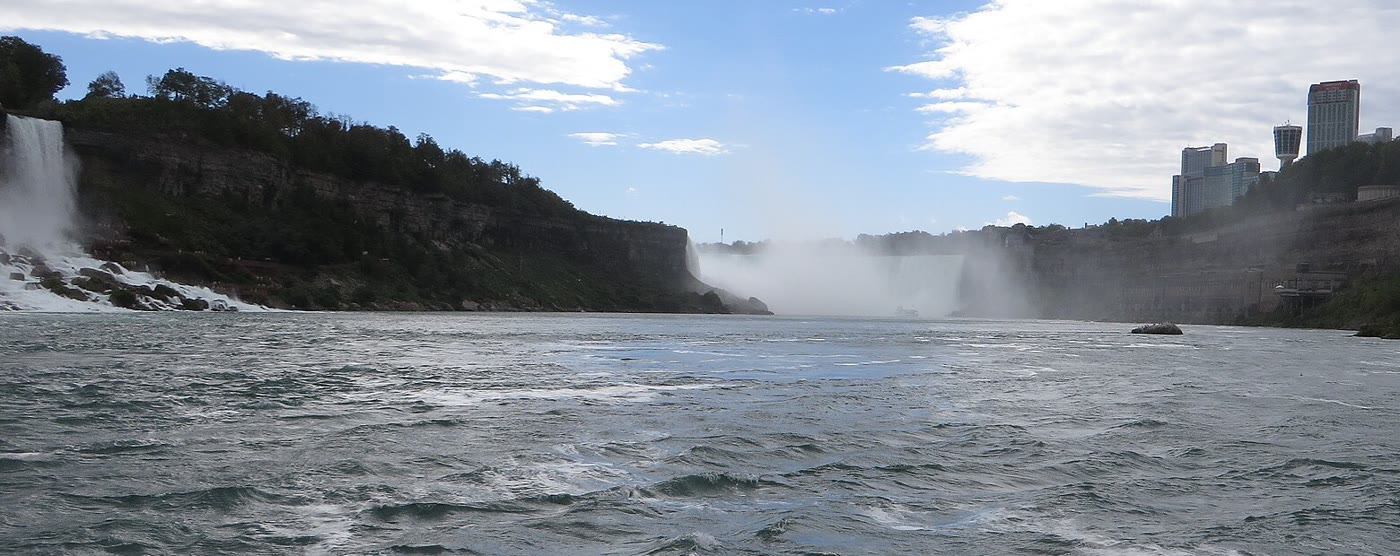
\includegraphics[width=\linewidth]{images/book5/b3-niagara-gorge.jpg}

{\scriptsize A Garganta do Niágara, vista rio acima até as Horseshoe Falls em
sua névoa, com as American Falls na borda esquerda. Foto de Ken Lund,
CC BY-SA 2.0 (recortada).}
\end{minipage}
\end{inthefield}
% ledger: ijc18:niagara, photo:b3-niagara-gorge


\section{Erosão glacial}\label{sec:b3:quantitative-geomorphology:glacial}

Uma geleira que desliza sobre seu leito (deslizamento basal,
Capítulo~\ref{ch:b3:glaciology}) erode-o por abrasão, com detritos retidos no
gelo, que raspam a rocha, e por arrancamento, quando arranca blocos afrouxados
por fissuras. Ambos variam com a velocidade de deslizamento.

\begin{definition}[Lei de erosão glacial]\label{def:b3:quantitative-geomorphology:glacial}
Uma \emph{lei de erosão glacial}\index{lei de erosão glacial} fornece a taxa de
erosão do leito de uma geleira como $E = K_G\,u_s^{\,l}$, em que $u_s$ é a
velocidade de deslizamento, $K_G$ um coeficiente e $l$ um expoente.
\end{definition}

Modelos de paisagem costumam adotar $l = 1$, mas usam-se valores entre 1 e 2.
Uma compilação de 38 geleiras, cujas taxas de erosão abrangem cinco ordens de
grandeza, encontrou erosão correlacionada com a velocidade de deslizamento, com $l = 0.65$ e
$K_G = 10^{-4}$ para $E$ em metros por ano: a erosão é mais rápida sob geleiras temperadas
alimentadas por neve abundante, que deslizam rapidamente. Como o gelo é mais espesso
e mais rápido ao longo do eixo de um vale, o fundo é aprofundado mais do que os
flancos, e o vale adquire sua forma de U.
% ledger: cook20:glacial

\begin{definition}[Serra circular glacial]\label{def:b3:quantitative-geomorphology:buzzsaw}
A \emph{serra circular glacial}\index{serra circular glacial} é o limite imposto à
altura de uma cadeia montanhosa pelas geleiras: onde a rocha se eleva acima da altitude
na qual as geleiras se formam, elas a erodem tão depressa quanto ela se eleva, qualquer que seja a
taxa de soerguimento, de modo que picos e altitude média se concentram perto dessa altitude.
\end{definition}

\section{Tectônica e erosão}\label{sec:b3:quantitative-geomorphology:tectonics}

\begin{definition}[Estado estacionário topográfico]\label{def:b3:quantitative-geomorphology:steady-state}
Uma paisagem está em \emph{estado estacionário topográfico}\index{estado estacionário topográfico}
quando sua taxa de erosão iguala em toda parte a taxa de soerguimento da rocha, de modo
que suas altitudes não mudam, embora a rocha passe por ela.
\end{definition}

Taxas medidas em intervalos de tempo diferentes testam esse estado. Os \omterm{def:b3:advanced-geochronology:cosmogenic}{nuclídeos cosmogênicos}
em areias de rio fornecem a taxa média de erosão de uma bacia ao longo do tempo
necessário para remover uma camada da ordem do comprimento de atenuação de sua
produção, cerca de \qty{55}{cm} de rocha; os \omterm{def:b3:orogenic-wedges:thermochronology}{termocronômetros} e suas relações idade--altitude fornecem a
taxa de exumação ao longo de milhões de anos. Onde as duas concordam entre si
e com a taxa de soerguimento, a paisagem provavelmente está em \omterm{def:b3:quantitative-geomorphology:steady-profile}{estado estacionário}; onde
a taxa de curto prazo é mais rápida nos trechos baixos do que nas cabeceiras,
um \omterm{def:b3:quantitative-geomorphology:knickpoint}{knickpoint} está passando. A remoção de rocha também alivia a
litosfera, que se eleva em resposta.
% ledger: zech04:exposure

\begin{definition}[Rebote isostático erosivo]\label{def:b3:quantitative-geomorphology:rebound}
O \emph{rebote isostático erosivo}\index{rebote isostático erosivo} é
a elevação da superfície rochosa de uma região em equilíbrio isostático em
resposta à massa removida pela erosão.
\end{definition}

\begin{proposition}[Os picos se elevam à medida que os vales se aprofundam]\label{prop:b3:quantitative-geomorphology:rebound}
Na isostasia de Airy, com crosta de densidade $\rho_c$ sobre manto de densidade
$\rho_m$, a remoção de uma espessura média $\bar e$ de crosta de uma região eleva
toda a região em $(\rho_c/\rho_m)\,\bar e$. Se a erosão se restringe
aos vales, os topos não erodidos se elevam nessa quantidade, enquanto a
superfície média desce apenas $(1 - \rho_c/\rho_m)\,\bar e$.
\end{proposition}

\begin{proof}
A compensação exige que a massa de cada coluna acima de uma profundidade fixa permaneça
a mesma. Remover uma espessura $\bar e$ de crosta, média sobre a área
de compensação, reduz a massa por unidade de área em $\rho_c \bar e$;
repô-la exige que o manto flua para dentro em profundidade, elevando a base da
coluna, e tudo o que está sobre ela, de $\delta$, com $\rho_m \delta = \rho_c \bar
e$. Um topo que não perdeu rocha eleva-se de $\delta$; a superfície média perde
$\bar e$ e ganha $\delta$.
\end{proof}

A densidade da crosta do modelo de referência da Terra, ponderada pela espessura, é
\qty{2.72}{g/cm^3} e a do manto abaixo de sua Moho \qty{3.38}{g/cm^3},
uma razão de 0.80: a cada cem metros de rocha erodida, a superfície média
perde apenas vinte. Um entalhe profundo de um planalto antigo pode, assim, elevar seus
topos mesmo enquanto o planalto se desgasta.
% ledger: prem:crust-mantle-ratio

\begin{omfigure}
\begin{tikzpicture}[x=0.6cm, y=0.6cm, font=\scriptsize]
\begin{scope}
\fill[omDef!12] (0,0) rectangle (8,4);
\draw[thick] (0,4) -- (8,4);
\draw[densely dashed] (0,0) -- (8,0);
\node[anchor=north] at (4,-0.1) {base da crosta};
\node at (4,2) {crosta $\rho_c$};
\node at (4,-1.2) {manto $\rho_m$};
\node[anchor=south] at (4,4.1) {antes};
\end{scope}
\begin{scope}[xshift=6.2cm]
\fill[omDef!12] (0,0.8) -- (0,4.8) -- (1.4,4.8) -- (2.0,2.4) -- (2.6,4.8) -- (5.4,4.8) -- (6.0,2.4) -- (6.6,4.8) -- (8,4.8) -- (8,0.8) -- cycle;
\draw[thick] (0,4.8) -- (1.4,4.8) -- (2.0,2.4) -- (2.6,4.8) -- (5.4,4.8) -- (6.0,2.4) -- (6.6,4.8) -- (8,4.8);
\draw[black!50, densely dashed] (0,4) -- (8,4);
\draw[densely dashed] (0,0.8) -- (8,0.8);
\draw[densely dashed, black!40] (0,0) -- (8,0);
\draw[<->, omThm] (8.3,4.05) -- (8.3,4.75) node[midway, right] {$\delta$};
\draw[<->, omThm] (8.3,0.05) -- (8.3,0.75) node[midway, right] {$\delta$};
\node[anchor=west, font=\scriptsize] at (8.1,2.4) {$\delta = (\rho_c/\rho_m)\,\bar e$};
\node[anchor=south] at (4,5.0) {após o entalhe dos vales};
\node[anchor=north] at (2.0,2.3) {vale};
\end{scope}
\end{tikzpicture}

\par\smallskip{\small \omterm{def:b3:quantitative-geomorphology:rebound}{Rebote isostático erosivo}, esquemático. O entalhe de
vales remove uma espessura média $\bar e$ de crosta; a coluna sobe em
$\delta = (\rho_c/\rho_m)\bar e$ na sua base e nos seus topos não erodidos
(a linha tracejada cinza é a superfície antiga).}\label{fig:b3:quantitative-geomorphology:rebound}
\end{omfigure}

\section{Exercícios}

\begin{exercise}[$\star$]\label{exo:b3:quantitative-geomorphology:1}
Uma escarpa litorânea de deslocamento \qty{4}{m} ($a = \qty{2}{m}$) situa-se sobre
um declive em campo distante de 0.04, e seu gradiente mais íngreme é agora 0.30. Calcule
$\kappa t$ e, em seguida, a idade da escarpa com $\kappa = \qty{5e-3}{m^2/yr}$.
\end{exercise}
% ledger: whipple04:scarp-erf, whipple04:scarp-kappa

\begin{exercise}[$\star$]\label{exo:b3:quantitative-geomorphology:2}
Um levantamento com lidar fornece uma curvatura de topo de \qty{-0.012}{m^{-1}} em uma crista
de difusividade \qty{4e-3}{m^2/yr}. Calcule sua taxa de erosão em
\unit{mm/yr}, e o relevo entre sua crista e os canais
a \qty{80}{m} de distância, supondo \omterm{def:b3:quantitative-geomorphology:steady-profile}{estado estacionário}.
\end{exercise}

\begin{exercise}[$\star$]\label{exo:b3:quantitative-geomorphology:3}
Com $m = 0.5$, $n = 1$ e $K = \qty{2e-6}{yr^{-1}}$, calcule a
taxa de entalhe de um rio que drena \qty{25}{km^2} com gradiente de 0.01.
Quais são as unidades de $K$ para $m$ e $n$ gerais?
\end{exercise}

\begin{exercise}[$\star$]\label{exo:b3:quantitative-geomorphology:4}
Três rios apresentam \textit{\omterm{def:b3:quantitative-geomorphology:knickpoint}{knickpoints}}: (a) onde um leito de arenito cruza um vale
entalhado em folhelho; (b) onde um rio cruza uma falha normal ativa, do
bloco inferior para o bloco superior; (c) em todos os rios de uma bacia, todos
na mesma altitude aproximada, a alguns quilômetros acima de uma costa que se
elevou em um terremoto. Quais são fixos e quais vão migrar?
\end{exercise}

\begin{exercise}[$\star\star$]\label{exo:b3:quantitative-geomorphology:5}
Para $m = 1$ e $n = 2$, calcule $\theta$ e o gradiente de \omterm{def:b3:quantitative-geomorphology:steady-profile}{estado estacionário} onde $A =
\qty{10}{km^2}$, com $U = \qty{0.1}{mm/yr}$ e $K = 10^{-9}$ em metros e
anos.
De que fator muda a declividade se $U$ dobrar? Compare com $n =
1$.
\end{exercise}

\begin{exercise}[$\star\star$]\label{exo:b3:quantitative-geomorphology:6}
A área de drenagem de um rio cresce com a distância $d$ de seu divisor como $A =
c\,d^{h}$. Mostre que, medido a montante de sua foz em $d = L$,
\[
\chi(d) = \frac{A_0^{\theta}}{c^{\theta}}\,\frac{L^{p} - d^{p}}{p},
\qquad p = 1 - h\theta ,
\]
e calcule-o para $c = 2$ (SI), $h = 1.8$, $\theta = 0.45$, $A_0 =
\qty{1}{km^2}$, $L = \qty{20}{km}$ e $d = \qty{5}{km}$.
\end{exercise}

\begin{exercise}[$\star\star$]\label{exo:b3:quantitative-geomorphology:7}
Com $n = 1$, $m = 0.5$ e $K = \qty{2e-6}{yr^{-1}}$, calcule a
celeridade de um \omterm{def:b3:quantitative-geomorphology:knickpoint}{knickpoint} onde $A = \qty{100}{km^2}$, em m/kyr, e o
tempo que levaria para percorrer \qty{5}{km} nessa velocidade. Por que ele
de fato leva mais tempo?
\end{exercise}

\begin{exercise}[$\star\star$]\label{exo:b3:quantitative-geomorphology:8}
Vales com \qty{600}{m} de profundidade, ocupando em média \qty{40}{\percent} da
área de um planalto, são entalhados nele. Com $\rho_c/\rho_m = 0.80$, calcule
a espessura média erodida, a elevação dos topos e a variação da
altitude média.
\end{exercise}
% ledger: prem:crust-mantle-ratio

\begin{exercise}[$\star\star$]\label{exo:b3:quantitative-geomorphology:9}
Uma \omterm{def:b3:quantitative-geomorphology:soil-production}{função de produção de solo} tem $P_0 = \qty{0.3}{mm/yr}$ e $h_0 =
\qty{0.5}{m}$. Calcule a espessura de solo em \omterm{def:b3:quantitative-geomorphology:steady-profile}{estado estacionário} para erosão de
\qty{0.05}{mm/yr} e de \qty{0.2}{mm/yr}. O que acontece com
\qty{0.4}{mm/yr}?
\end{exercise}

\begin{exercise}[$\star\star\star$]\label{exo:b3:quantitative-geomorphology:10}
Uma colina em \omterm{def:b3:quantitative-geomorphology:steady-profile}{estado estacionário} erode a $E = \qty{0.1}{mm/yr}$ com $\kappa =
\qty{5e-3}{m^2/yr}$ e a lei não linear do gradiente crítico, adotando
$S_c = 1.2$ para o exercício. Mostre que o fluxo a uma distância $x$ do
divisor é $E x$, resolva para o gradiente e calcule-o em 20, 50, 100 e
\qty{200}{m}. Compare com a difusão linear e descreva a forma da
colina.
\end{exercise}

\begin{exercise}[$\star\star\star$]\label{exo:b3:quantitative-geomorphology:11}
Mostre que o tempo de resposta de uma rede de drenagem a uma mudança em sua foz,
para $n = 1$, é $\chi_h/(K A_0^m)$, em que $\chi_h$ é o maior valor de
$\chi$ em uma cabeceira de canal. Calcule-o para o rio de planalto das figuras
($A_0 = \qty{1}{km^2}$, $m = 0.5$, $K = \qty{e-6}{yr^{-1}}$), primeiro para seu
tronco isoladamente, cuja cabeceira está em $\chi = \qty{5464}{m}$, depois para a rede,
cuja cabeceira mais alta, no afluente 1, está em $\chi = \qty{7237}{m}$.
\end{exercise}

\begin{exercise}[$\star\star\star$]\label{exo:b3:quantitative-geomorphology:12}
Em uma rede com $n = 1$ e $U$ uniforme, um afluente escoa sobre rocha duas
vezes mais erodível que o restante ($2K$) acima de sua confluência, em $\chi_j$. Mostre que
sua linha de \omterm{def:b3:quantitative-geomorphology:steady-profile}{estado estacionário} no plano $(\chi, z)$ tem metade da inclinação da
do tronco acima de $\chi_j$, e que um \omterm{def:b3:quantitative-geomorphology:knickpoint}{knickpoint} originado na foz atinge,
no instante em que o \omterm{def:b3:quantitative-geomorphology:knickpoint}{knickpoint} do tronco está em $\chi_k > \chi_j$, o ponto
de $\chi = \chi_j + 2(\chi_k - \chi_j)$ desse afluente.
\end{exercise}

\section{Problema: A cachoeira do rio Varden}

\begin{problem}[{Problema de fim de semana --- o perfil, a declividade e a erodibilidade
de um rio de planalto fictício, e a idade de sua cachoeira}]
\label{pb:b3:quantitative-geomorphology:1}
A oeste das Varden Hills, o rio drena um planalto de xisto antes de
entrar no mapa por sua borda oeste, a uma altitude de \qty{170}{m}. A montante
desse ponto, sua foz, o tronco tem \qty{12}{km} de comprimento a partir de seu divisor,
com área de drenagem $A = 4.5\,d^{1.7}$ (\unit{m^2}, $d$ em metros a partir do
divisor) e uma cabeceira de canal em $d = \qty{300}{m}$. Tome como taxa de
soerguimento rochoso a taxa de denudação da bacia do rio Varden, obtida a partir de suas cargas
no volume do primeiro ano, \qty{43}{m/Myr}. Tome $n = 1$ e a área de referência $A_0 = \qty{1}{km^2}$.
Uma cachoeira de \qty{25}{m} de altura situa-se no tronco a \qty{4.60}{km} a montante
da foz. Todos os valores são fictícios.

\medskip\noindent\textbf{Parte I --- O perfil.}
\begin{enumerate}
\item Calcule a área de drenagem na foz e na cabeceira do canal.
\item Gradientes medidos em trechos de \qty{200}{m}, afastados da
  cachoeira:

  \smallskip
  {\small\begin{tabular}{l*{6}{c}}
  $A$ (\unit{km^2}) & 0.388 & 0.587 & 0.888 & 1.345 & 2.036 & 3.082 \\
  $S$ & 0.06641 & 0.05026 & 0.04888 & 0.03322 & 0.03688 & 0.02688 \\[2pt]
  $A$ (\unit{km^2}) & 4.665 & 7.061 & 10.69 & 16.18 & 24.49 & 37.08 \\
  $S$ & 0.01921 & 0.01713 & 0.01545 & 0.01419 & 0.007922 & 0.007855
  \end{tabular}}

  \smallskip
  Estime o \omterm{def:b3:quantitative-geomorphology:indices}{índice de concavidade} a partir do primeiro e do último ponto.
\item A inclinação de mínimos quadrados de $\log S$ em função de $\log A$ é $-0.466$.
  Esse valor é compatível com $\theta = 0.5$?
\item Com $\theta_{\mathrm{ref}} = 0.5$, calcule $k_{sn} = S A^{0.5}$ ($A$ em
  \unit{m^2}) para o primeiro e o último ponto, e diga o que representa a
  média geométrica dos doze valores, \qty{45.1}{m}.
\item Por que os gradientes se dispersam muito mais do que as altitudes?
\item Usando a fórmula do exercício de chi, calcule $\chi$ em $d =
  \qty{9.00}{km}$, um ponto abaixo da cachoeira.
\end{enumerate}

\medskip\noindent\textbf{Parte II --- Declividade e erodibilidade.}
\begin{enumerate}[resume]
\item O rio está em \qty{193.4}{m} em $d = \qty{9.00}{km}$. Calcule a
  inclinação do gráfico de chi abaixo da cachoeira e a declividade $k_{sn}$.
\item Qual das estimativas de $k_{sn}$, esta ou a da declividade--área, é mais
  confiável, e por quê?
\item Supondo \omterm{def:b3:quantitative-geomorphology:steady-profile}{estado estacionário} abaixo da cachoeira, calcule $K$ a partir da
  taxa de soerguimento.
\item Verifique que a taxa de entalhamento na foz, cujo gradiente é
  0.00691, é igual à taxa de soerguimento.
\item Calcule a celeridade de um \omterm{def:b3:quantitative-geomorphology:knickpoint}{knickpoint} na foz e na
  cachoeira, em m/kyr.
\item Calcule a altitude da cabeceira do canal no perfil em \omterm{def:b3:quantitative-geomorphology:steady-profile}{estado estacionário}, e o
  relevo do tronco.
\end{enumerate}

\medskip\noindent\textbf{Parte III --- A cachoeira.}
\begin{enumerate}[resume]
\item Por que, com $n = 1$, a cachoeira manteve a altura da queda do
  \omterm{def:b3:quantitative-geomorphology:knickpoint}{nível de base}?
\item Calcule $\chi$ na cachoeira.
\item Calcule o tempo que o \omterm{def:b3:quantitative-geomorphology:knickpoint}{knickpoint} levou da foz até sua
  posição atual.
\item Onde ele estará daqui a \qty{300}{kyr}?
\item O afluente 3 se une ao tronco a \qty{2.5}{km} a montante da foz; ele
  tem \qty{5}{km} de comprimento, com $A = 1.5\,s^{1.7}$ ($s$ medido a partir de seu próprio divisor).
  Onde deve estar sua cachoeira?
\item Os afluentes 1 e 2 se unem ao tronco a 8 e \qty{5}{km} a montante da
  foz. Explique por que eles não têm cachoeira.
\end{enumerate}

\medskip\noindent\textbf{Parte IV --- As encostas e a idade.}
\begin{enumerate}[resume]
\item Um levantamento lidar acima da cachoeira fornece uma curvatura no
  topo das colinas de \qty{-0.0086}{m^{-1}}. Com $\kappa = \qty{5e-3}{m^2/yr}$, calcule a
  taxa de erosão e compare-a com a taxa de soerguimento.
\item As encostas têm cerca de \qty{150}{m} de comprimento. Compare seu tempo de resposta
  $L^2/\kappa$ com a idade obtida na Parte III.
\item Descreva as encostas abaixo da cachoeira hoje, e como elas
  vão mudar.
\item A taxa de soerguimento é conhecida com incerteza de \qty{20}{\percent}. Dê a
  faixa de valores da idade.
\item Como a cachoeira teria evoluído se $n$ fosse 2?
\item Dê a idade da queda do \omterm{def:b3:quantitative-geomorphology:knickpoint}{nível de base}.
\end{enumerate}
\end{problem}
% ledger: whipple04:steepness, whipple04:scarp-kappa
